\section{Design}
\label{sec:design}

\begin{figure*}[tbhp]
  \centering
  \begin{subfigure}[b]{1.0\linewidth}
    \centering
    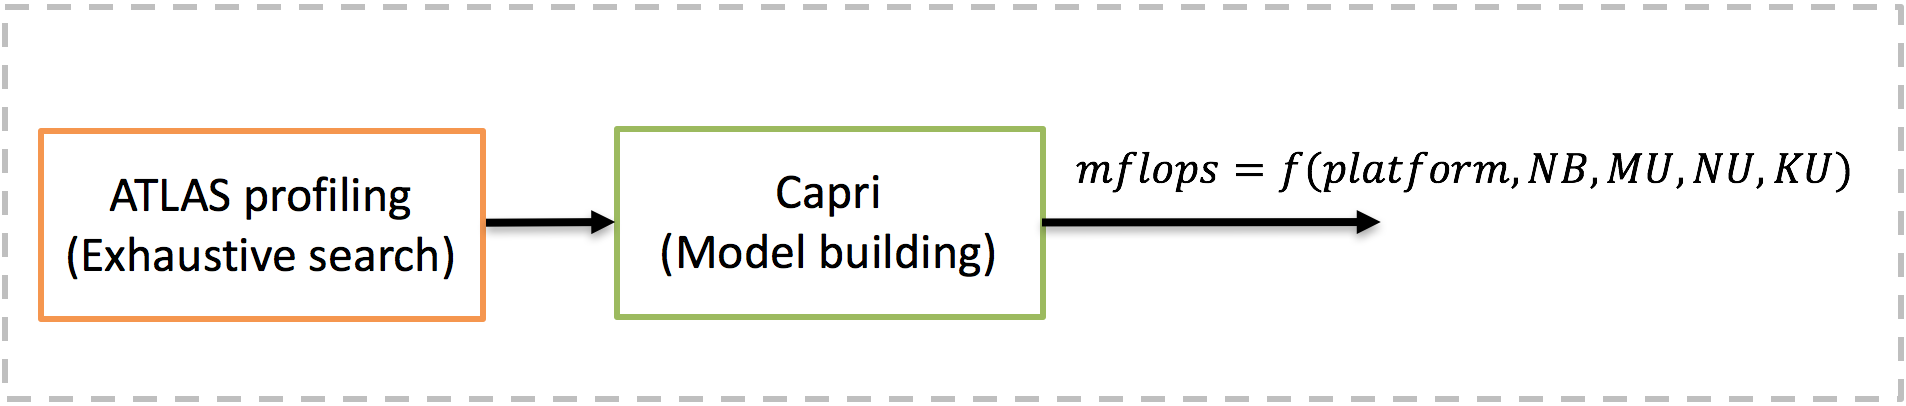
\includegraphics[width=0.9\textwidth]{images/offline_training.png}
    \caption{Offline training phase: \atl profiling and Capri model building}
    \label{fig:design_train}
  \end{subfigure}
  \begin{subfigure}[b]{1.0\linewidth}
    \centering
    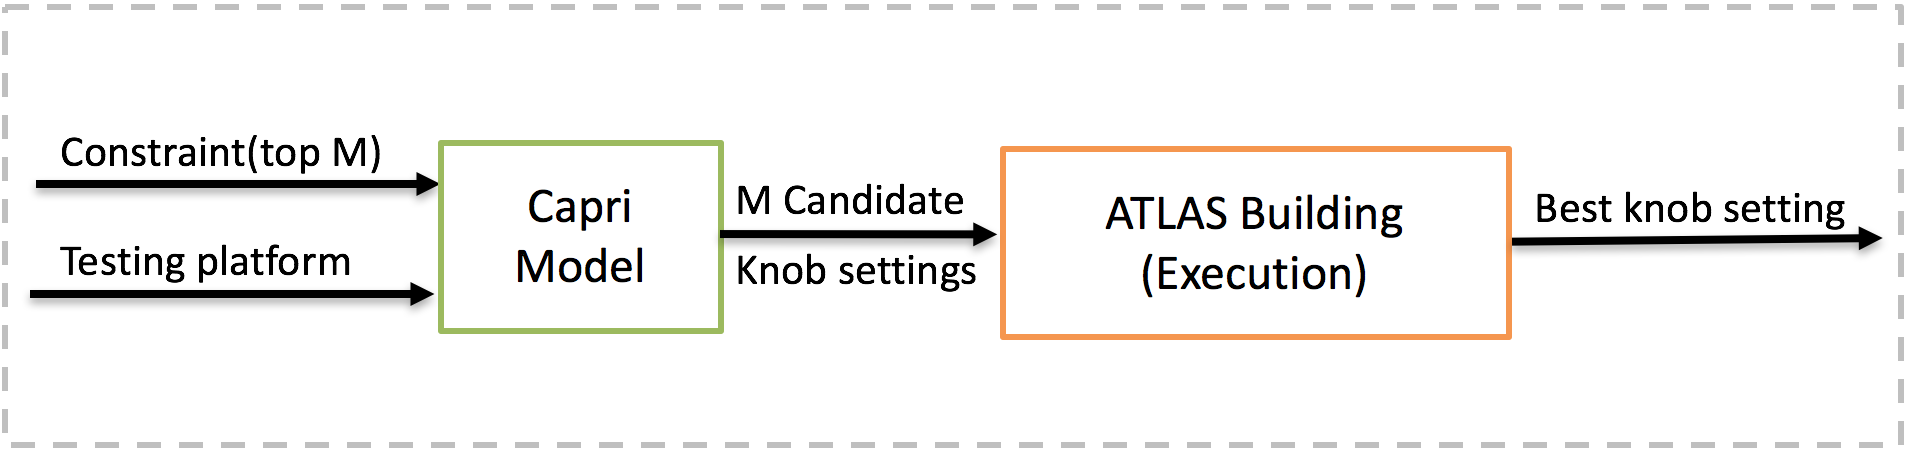
\includegraphics[width=0.9\textwidth]{images/testing.png}
    \caption{Online testing phase: Capri model searching and \atl execution}
    \label{fig:design_test}
  \end{subfigure}
  \caption{Capri-based \atl design diagram}
\end{figure*}

As mentioned in the motivation section, the orthogonal searching strategy used in 
\atl is quite problematic. It can only generate good results for some platforms
and the install process is slow. The high level idea to speed up \atl
optimization process as well as improving \gem performance is to replace the
original searching space by the new space generated by Capri.

The design of our Capri-based \atl can be separated into four parts: knob
selection, feature selection, the offline training phase and the online testing
phase. One \atl installation process generates linear algebra libraries for one
platform. Hence, the input to Capri is a particular platform. Some features are
extracted to represent the platform, such as type of cores, core frequency and
so on. Knobs, as descried in Section~\ref{sec:Capri_intro}, affects the
performance of any input of a target application. The offline training phase
captures the characteristics of the platform features and knob settings by doing
exhaustive runs. Capri uses the profiling data generated by exhaustive runs and
builds a model for the \gem performance. In the testing phase, the model takes
a platform and a ``top M'' constraint as input, and output the best predicted
knob setting for GEMM for this platform.

The detailed design are descried in the following for subsections.

  \subsection{Knob selection}
  \label{sec:knobs}
  As mentioned in Section~\ref{sec:atlas_intro}, \atl optimizes a set of knobs
  including {$NB$, $MU$, $NU$, $KU$, $L_s$, $FMA$, $F_F$, $I_F$, $N_F$} by
  using orthogonal search. Altogether there are 9 knobs here. $NB$, $MU$, $NU$
  and $KU$ have roughly 10$\sim$20 configurable settings respectively, $L_s$,
  $F_F$, $I_F$ and $N_F$ have roughly 5$\sim$10 different settings respectively.
  $FMA$ has 2 settings. If all knobs are considered in the offline profiling
  process, the searching space is over 100 million for one platform, which is
  obviously inapplicable in reality. Based on some careful study of the
  effect of knobs on \gem performance, we found out that only $NB$, $MU$, $NU$
  and $KU$ has significant effect on the performance, while other knobs only
  have minor($\sim$10\%) effect. Therefore, we choose $NB$, $MU$, $NU$ and $KU$
  as our knob space. The size of the joint space is around 12500, most
  platforms can finish these many runs in one day.

  \subsection{Feature selection}
  \label{sec:features}
  Features are used in Capri as the identification for different inputs. In this
  project, obviously platform features affects a lot. For example, processors
  from \emph{Intel, ARM} or \emph{AMD} performs really differently even with
  the some clock frequency. Or another example, performance on MAC OS and Linux
  are very different because the compiler used to generate code is very
  different. By inspecting \atl configuration step, we choose 6 features as the
  indicators of one platform. We cannot tell the exact effect of each feature
  but the machine learning model can.
  \begin{itemize}
  \item Architecture categorized by \atl
  \item Compiler type
  \item Number of registers
  \item Size of the L1 instruction cache
  \item CPU frequency
  \item CPU benchmark performance\footnote{CPU score given by
  https://www.cpubenchmark.net/cpu\_list.php}
  \end{itemize}

  \subsection{Offline Training}
  \label{sec:offline_training}
  The diagram of the offline training phase is shown in
  Fig.\ref{fig:design_train}. An interface is implemented in \atl in order to
  take knob settings as input, generate code and evaluate the performance of
  the input knob setting. The design space for each training platform is
  constrained by $NB$, $MU$, $NU$ and $KU$. For each knob setting in the space,
  its performance will be evaluated on each platform. All the knob-performance
  pairs generated by all the training platforms, together with their platform
  features, will be fed into the Capri model building module. The function of
  the model is expressed in Equation~\ref{equ:model_func}. This \emph{Perf}
  model takes platform features, $NB$, $MU$, $NU$ and $KU$ as inputs and
  provides a predicted performance.

  \begin{equation}
  \label{equ:model_func}
  mflops = \textbf{Perf}{(platform, NB, MU, NU, KU)}
  \end{equation}

  \subsection{Online Testing}
  \label{sec:online_testing}
  The online testing part is the new install process for \atl, as shown in
  Fig~\ref{fig:design_test}. The newly built performance model takes a new
  platform and a ``top M'' constraint as input. Along with the platform
  features, each knob is fed into the \emph{Perf} model in order to find the
  top M knob setting candidates by actually consulting the model and find its
  predicted performance. Then, the actual performance of the top M
  knob setting candidates will be evaluated exhaustively by \atl. Finally,
  the knob setting with the best actual performance will be used to
  generate the executable.

  \subsection{Machine Learning Model}
  \label{sec:matching_learning_model}
  There different kinds of machine learning model implemented in Capri. In
  thie paper, we mainly choose three decision tree style model, which are
  M5~\cite{quinlan1992learning}, bagging predictor~\cite{breiman1996bagging}
  and extremely randomized trees~\cite{geurts2006extremely}. M5 can be
  understood as piecewise linear regressor by linearly divide the knob space.
  Bagging predictors is a method for generating multiple versions of a
  predictor and using these to get an aggregated predictor. The aggregation
  averages over the versions when predicting a numerical outcome and does
  plurality vote when predicting a class. Extremely randomized trees are
  trees-based ensemble method for supervised classification and regression
  problems. It essentially consists of randomizing strongly both attribute
  and cut-point choice while splitting a tree node. These three decision trees
  are enough powerful to model the performance of \gem while they are quite
  easy to evaluate and not heavily parameter dependent compared to
  deep neural network methods.
